% Options for packages loaded elsewhere
\PassOptionsToPackage{unicode}{hyperref}
\PassOptionsToPackage{hyphens}{url}
\PassOptionsToPackage{dvipsnames,svgnames,x11names}{xcolor}
%
\documentclass[
  letterpaper,
  DIV=11,
  numbers=noendperiod]{scrartcl}

\usepackage{amsmath,amssymb}
\usepackage{iftex}
\ifPDFTeX
  \usepackage[T1]{fontenc}
  \usepackage[utf8]{inputenc}
  \usepackage{textcomp} % provide euro and other symbols
\else % if luatex or xetex
  \usepackage{unicode-math}
  \defaultfontfeatures{Scale=MatchLowercase}
  \defaultfontfeatures[\rmfamily]{Ligatures=TeX,Scale=1}
\fi
\usepackage{lmodern}
\ifPDFTeX\else  
    % xetex/luatex font selection
\fi
% Use upquote if available, for straight quotes in verbatim environments
\IfFileExists{upquote.sty}{\usepackage{upquote}}{}
\IfFileExists{microtype.sty}{% use microtype if available
  \usepackage[]{microtype}
  \UseMicrotypeSet[protrusion]{basicmath} % disable protrusion for tt fonts
}{}
\makeatletter
\@ifundefined{KOMAClassName}{% if non-KOMA class
  \IfFileExists{parskip.sty}{%
    \usepackage{parskip}
  }{% else
    \setlength{\parindent}{0pt}
    \setlength{\parskip}{6pt plus 2pt minus 1pt}}
}{% if KOMA class
  \KOMAoptions{parskip=half}}
\makeatother
\usepackage{xcolor}
\setlength{\emergencystretch}{3em} % prevent overfull lines
\setcounter{secnumdepth}{-\maxdimen} % remove section numbering
% Make \paragraph and \subparagraph free-standing
\makeatletter
\ifx\paragraph\undefined\else
  \let\oldparagraph\paragraph
  \renewcommand{\paragraph}{
    \@ifstar
      \xxxParagraphStar
      \xxxParagraphNoStar
  }
  \newcommand{\xxxParagraphStar}[1]{\oldparagraph*{#1}\mbox{}}
  \newcommand{\xxxParagraphNoStar}[1]{\oldparagraph{#1}\mbox{}}
\fi
\ifx\subparagraph\undefined\else
  \let\oldsubparagraph\subparagraph
  \renewcommand{\subparagraph}{
    \@ifstar
      \xxxSubParagraphStar
      \xxxSubParagraphNoStar
  }
  \newcommand{\xxxSubParagraphStar}[1]{\oldsubparagraph*{#1}\mbox{}}
  \newcommand{\xxxSubParagraphNoStar}[1]{\oldsubparagraph{#1}\mbox{}}
\fi
\makeatother

\usepackage{color}
\usepackage{fancyvrb}
\newcommand{\VerbBar}{|}
\newcommand{\VERB}{\Verb[commandchars=\\\{\}]}
\DefineVerbatimEnvironment{Highlighting}{Verbatim}{commandchars=\\\{\}}
% Add ',fontsize=\small' for more characters per line
\usepackage{framed}
\definecolor{shadecolor}{RGB}{241,243,245}
\newenvironment{Shaded}{\begin{snugshade}}{\end{snugshade}}
\newcommand{\AlertTok}[1]{\textcolor[rgb]{0.68,0.00,0.00}{#1}}
\newcommand{\AnnotationTok}[1]{\textcolor[rgb]{0.37,0.37,0.37}{#1}}
\newcommand{\AttributeTok}[1]{\textcolor[rgb]{0.40,0.45,0.13}{#1}}
\newcommand{\BaseNTok}[1]{\textcolor[rgb]{0.68,0.00,0.00}{#1}}
\newcommand{\BuiltInTok}[1]{\textcolor[rgb]{0.00,0.23,0.31}{#1}}
\newcommand{\CharTok}[1]{\textcolor[rgb]{0.13,0.47,0.30}{#1}}
\newcommand{\CommentTok}[1]{\textcolor[rgb]{0.37,0.37,0.37}{#1}}
\newcommand{\CommentVarTok}[1]{\textcolor[rgb]{0.37,0.37,0.37}{\textit{#1}}}
\newcommand{\ConstantTok}[1]{\textcolor[rgb]{0.56,0.35,0.01}{#1}}
\newcommand{\ControlFlowTok}[1]{\textcolor[rgb]{0.00,0.23,0.31}{\textbf{#1}}}
\newcommand{\DataTypeTok}[1]{\textcolor[rgb]{0.68,0.00,0.00}{#1}}
\newcommand{\DecValTok}[1]{\textcolor[rgb]{0.68,0.00,0.00}{#1}}
\newcommand{\DocumentationTok}[1]{\textcolor[rgb]{0.37,0.37,0.37}{\textit{#1}}}
\newcommand{\ErrorTok}[1]{\textcolor[rgb]{0.68,0.00,0.00}{#1}}
\newcommand{\ExtensionTok}[1]{\textcolor[rgb]{0.00,0.23,0.31}{#1}}
\newcommand{\FloatTok}[1]{\textcolor[rgb]{0.68,0.00,0.00}{#1}}
\newcommand{\FunctionTok}[1]{\textcolor[rgb]{0.28,0.35,0.67}{#1}}
\newcommand{\ImportTok}[1]{\textcolor[rgb]{0.00,0.46,0.62}{#1}}
\newcommand{\InformationTok}[1]{\textcolor[rgb]{0.37,0.37,0.37}{#1}}
\newcommand{\KeywordTok}[1]{\textcolor[rgb]{0.00,0.23,0.31}{\textbf{#1}}}
\newcommand{\NormalTok}[1]{\textcolor[rgb]{0.00,0.23,0.31}{#1}}
\newcommand{\OperatorTok}[1]{\textcolor[rgb]{0.37,0.37,0.37}{#1}}
\newcommand{\OtherTok}[1]{\textcolor[rgb]{0.00,0.23,0.31}{#1}}
\newcommand{\PreprocessorTok}[1]{\textcolor[rgb]{0.68,0.00,0.00}{#1}}
\newcommand{\RegionMarkerTok}[1]{\textcolor[rgb]{0.00,0.23,0.31}{#1}}
\newcommand{\SpecialCharTok}[1]{\textcolor[rgb]{0.37,0.37,0.37}{#1}}
\newcommand{\SpecialStringTok}[1]{\textcolor[rgb]{0.13,0.47,0.30}{#1}}
\newcommand{\StringTok}[1]{\textcolor[rgb]{0.13,0.47,0.30}{#1}}
\newcommand{\VariableTok}[1]{\textcolor[rgb]{0.07,0.07,0.07}{#1}}
\newcommand{\VerbatimStringTok}[1]{\textcolor[rgb]{0.13,0.47,0.30}{#1}}
\newcommand{\WarningTok}[1]{\textcolor[rgb]{0.37,0.37,0.37}{\textit{#1}}}

\providecommand{\tightlist}{%
  \setlength{\itemsep}{0pt}\setlength{\parskip}{0pt}}\usepackage{longtable,booktabs,array}
\usepackage{calc} % for calculating minipage widths
% Correct order of tables after \paragraph or \subparagraph
\usepackage{etoolbox}
\makeatletter
\patchcmd\longtable{\par}{\if@noskipsec\mbox{}\fi\par}{}{}
\makeatother
% Allow footnotes in longtable head/foot
\IfFileExists{footnotehyper.sty}{\usepackage{footnotehyper}}{\usepackage{footnote}}
\makesavenoteenv{longtable}
\usepackage{graphicx}
\makeatletter
\newsavebox\pandoc@box
\newcommand*\pandocbounded[1]{% scales image to fit in text height/width
  \sbox\pandoc@box{#1}%
  \Gscale@div\@tempa{\textheight}{\dimexpr\ht\pandoc@box+\dp\pandoc@box\relax}%
  \Gscale@div\@tempb{\linewidth}{\wd\pandoc@box}%
  \ifdim\@tempb\p@<\@tempa\p@\let\@tempa\@tempb\fi% select the smaller of both
  \ifdim\@tempa\p@<\p@\scalebox{\@tempa}{\usebox\pandoc@box}%
  \else\usebox{\pandoc@box}%
  \fi%
}
% Set default figure placement to htbp
\def\fps@figure{htbp}
\makeatother
% definitions for citeproc citations
\NewDocumentCommand\citeproctext{}{}
\NewDocumentCommand\citeproc{mm}{%
  \begingroup\def\citeproctext{#2}\cite{#1}\endgroup}
\makeatletter
 % allow citations to break across lines
 \let\@cite@ofmt\@firstofone
 % avoid brackets around text for \cite:
 \def\@biblabel#1{}
 \def\@cite#1#2{{#1\if@tempswa , #2\fi}}
\makeatother
\newlength{\cslhangindent}
\setlength{\cslhangindent}{1.5em}
\newlength{\csllabelwidth}
\setlength{\csllabelwidth}{3em}
\newenvironment{CSLReferences}[2] % #1 hanging-indent, #2 entry-spacing
 {\begin{list}{}{%
  \setlength{\itemindent}{0pt}
  \setlength{\leftmargin}{0pt}
  \setlength{\parsep}{0pt}
  % turn on hanging indent if param 1 is 1
  \ifodd #1
   \setlength{\leftmargin}{\cslhangindent}
   \setlength{\itemindent}{-1\cslhangindent}
  \fi
  % set entry spacing
  \setlength{\itemsep}{#2\baselineskip}}}
 {\end{list}}
\usepackage{calc}
\newcommand{\CSLBlock}[1]{\hfill\break\parbox[t]{\linewidth}{\strut\ignorespaces#1\strut}}
\newcommand{\CSLLeftMargin}[1]{\parbox[t]{\csllabelwidth}{\strut#1\strut}}
\newcommand{\CSLRightInline}[1]{\parbox[t]{\linewidth - \csllabelwidth}{\strut#1\strut}}
\newcommand{\CSLIndent}[1]{\hspace{\cslhangindent}#1}

\usepackage{fvextra}
\DefineVerbatimEnvironment{Highlighting}{Verbatim}{breaklines,commandchars=\\\{\}}
\DefineVerbatimEnvironment{OutputCode}{Verbatim}{breaklines,commandchars=\\\{\}}
\KOMAoption{captions}{tableheading}
\makeatletter
\@ifpackageloaded{caption}{}{\usepackage{caption}}
\AtBeginDocument{%
\ifdefined\contentsname
  \renewcommand*\contentsname{Table of contents}
\else
  \newcommand\contentsname{Table of contents}
\fi
\ifdefined\listfigurename
  \renewcommand*\listfigurename{List of Figures}
\else
  \newcommand\listfigurename{List of Figures}
\fi
\ifdefined\listtablename
  \renewcommand*\listtablename{List of Tables}
\else
  \newcommand\listtablename{List of Tables}
\fi
\ifdefined\figurename
  \renewcommand*\figurename{Figure}
\else
  \newcommand\figurename{Figure}
\fi
\ifdefined\tablename
  \renewcommand*\tablename{Table}
\else
  \newcommand\tablename{Table}
\fi
}
\@ifpackageloaded{float}{}{\usepackage{float}}
\floatstyle{ruled}
\@ifundefined{c@chapter}{\newfloat{codelisting}{h}{lop}}{\newfloat{codelisting}{h}{lop}[chapter]}
\floatname{codelisting}{Listing}
\newcommand*\listoflistings{\listof{codelisting}{List of Listings}}
\makeatother
\makeatletter
\makeatother
\makeatletter
\@ifpackageloaded{caption}{}{\usepackage{caption}}
\@ifpackageloaded{subcaption}{}{\usepackage{subcaption}}
\makeatother

\usepackage{bookmark}

\IfFileExists{xurl.sty}{\usepackage{xurl}}{} % add URL line breaks if available
\urlstyle{same} % disable monospaced font for URLs
\hypersetup{
  pdftitle={PS 2},
  pdfauthor={Hyoungchul Kim},
  colorlinks=true,
  linkcolor={blue},
  filecolor={Maroon},
  citecolor={Blue},
  urlcolor={Blue},
  pdfcreator={LaTeX via pandoc}}


\title{PS 2}
\author{Hyoungchul Kim}
\date{2025-04-05}

\begin{document}
\maketitle


\section{Part 1}\label{part-1}

First, read in the data

\begin{Shaded}
\begin{Highlighting}[]
\FunctionTok{library}\NormalTok{(tidyverse)}
\FunctionTok{library}\NormalTok{(data.table)}

\NormalTok{data }\OtherTok{\textless{}{-}} \FunctionTok{read\_csv}\NormalTok{(}\StringTok{"data/middle\_kink.csv"}\NormalTok{)}

\CommentTok{\# view the data}
\NormalTok{data }\SpecialCharTok{\%\textgreater{}\%} \FunctionTok{head}\NormalTok{()}
\end{Highlighting}
\end{Shaded}

\begin{verbatim}
# A tibble: 6 x 2
  income_bin     n
       <dbl> <dbl>
1     151250   955
2     153750   982
3     156250   894
4     158750   873
5     161250   810
6     163750   851
\end{verbatim}

\subsection{a.}\label{a.}

Now we will plot the publication-quality histogram of the earnings
distribution:

\begin{Shaded}
\begin{Highlighting}[]
\FunctionTok{library}\NormalTok{(ggtext) }

\NormalTok{earning\_dist }\OtherTok{\textless{}{-}}\NormalTok{ data }\SpecialCharTok{\%\textgreater{}\%} 
  \FunctionTok{ggplot}\NormalTok{(}\FunctionTok{aes}\NormalTok{(}\AttributeTok{x=}\NormalTok{income\_bin, }\AttributeTok{y =}\NormalTok{ n)) }\SpecialCharTok{+}
  \FunctionTok{geom\_col}\NormalTok{(}\AttributeTok{fill =} \StringTok{"lightblue"}\NormalTok{) }\SpecialCharTok{+}
  \FunctionTok{geom\_point}\NormalTok{() }\SpecialCharTok{+}
  \CommentTok{\# geom\_smooth(method = "lm", se = FALSE, color = "black") +}
  \FunctionTok{geom\_line}\NormalTok{() }\SpecialCharTok{+}
  \FunctionTok{scale\_x\_continuous}\NormalTok{(}\AttributeTok{labels =}\NormalTok{ scales}\SpecialCharTok{::}\FunctionTok{label\_number}\NormalTok{(}\AttributeTok{scale =} \FloatTok{0.001}\NormalTok{, }\AttributeTok{prefix =} \StringTok{"$"}\NormalTok{)) }\SpecialCharTok{+}
  \FunctionTok{geom\_vline}\NormalTok{(}\AttributeTok{xintercept =} \DecValTok{363750}\NormalTok{, }\AttributeTok{color=}\StringTok{"red"}\NormalTok{, }\AttributeTok{shape=}\StringTok{"solid"}\NormalTok{) }\SpecialCharTok{+}
  \CommentTok{\# annotate("text", label = "kink", x = 380000, y = 800, size = 5, colour = "black") +}
  \FunctionTok{labs}\NormalTok{(}\AttributeTok{title =} \StringTok{"**Histogram of the earnings distribution**"}\NormalTok{,}
       \AttributeTok{x =} \StringTok{"**Income Bin (1000s)**"}\NormalTok{, }
       \AttributeTok{y =} \StringTok{"**Number of Observations**"}\NormalTok{) }\SpecialCharTok{+}
  \FunctionTok{theme\_bw}\NormalTok{() }\SpecialCharTok{+} 
  \FunctionTok{theme}\NormalTok{(}
    \AttributeTok{plot.title =} \FunctionTok{element\_markdown}\NormalTok{(}\AttributeTok{size =} \DecValTok{16}\NormalTok{, }\AttributeTok{hjust =} \FloatTok{0.5}\NormalTok{),}
    \AttributeTok{axis.title.x =} \FunctionTok{element\_markdown}\NormalTok{(}\AttributeTok{size =} \DecValTok{14}\NormalTok{),}
    \AttributeTok{axis.title.y =} \FunctionTok{element\_markdown}\NormalTok{(}\AttributeTok{size =} \DecValTok{14}\NormalTok{),}
    \AttributeTok{axis.text.x =} \FunctionTok{element\_text}\NormalTok{(}\AttributeTok{size =} \DecValTok{12}\NormalTok{),}
    \AttributeTok{axis.text.y =} \FunctionTok{element\_text}\NormalTok{(}\AttributeTok{size =} \DecValTok{12}\NormalTok{)}
\NormalTok{  )}
\NormalTok{earning\_dist}
\end{Highlighting}
\end{Shaded}

\pandocbounded{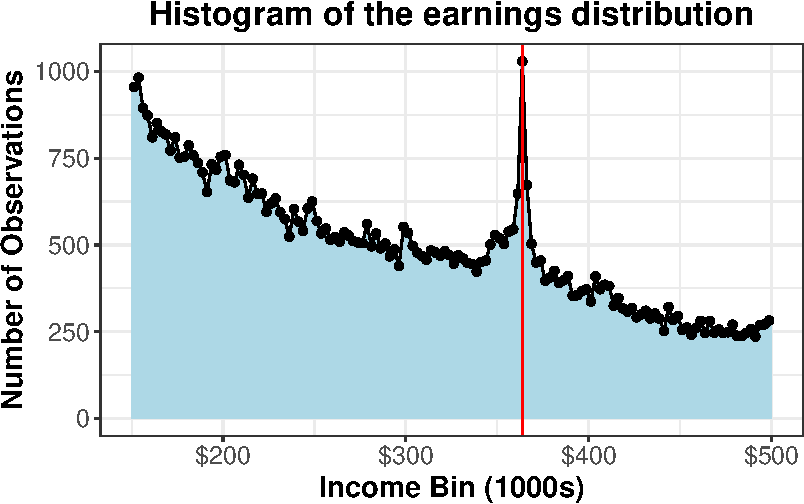
\includegraphics[keepaspectratio]{report_files/figure-pdf/unnamed-chunk-2-1.pdf}}

\subsection{b.}\label{b.}

We will be following Saez (2010) to construct the equation to retrieve
the elasticity \(e\). Note for our case, the kink happens as
\(z^* = 363750\) and marginal tax rate changes from \(0.21\) to
\(0.28\). We need to use equation (5) in the paper to get the
elasticity. The equation is as follows:

\[
  B = z^* \left[ \left( \frac{1-t_0}{1-t_1} \right)^e - 1 \right] \frac{h(z^*)\_ + h(z^*)_+ \bigg/ \left( \frac{1-t_0}{1-t_1} \right)^e}{2}.
\]

In order to compute \(B\), we need to decide \(\delta\) to calculate the
width we will use to calculate excess bunching. We will use the
``simplest method'' mentioned in the paper which is to select \(\delta\)
graphically such that the full excess bunching is included in the band
\((z^* - \delta + z^* + \delta)\). In our case, it seems to be about
\(\delta = 8\) (Note that since out data is in income bin of width 2500,
this is equivalent to 20,000 difference). Numerically, it will be
calculated as follows (this is just following the equation (6) in the
paper):

\begin{Shaded}
\begin{Highlighting}[]
\NormalTok{B1  }\OtherTok{\textless{}{-}}\NormalTok{ data }\SpecialCharTok{\%\textgreater{}\%} 
  \FunctionTok{filter}\NormalTok{(income\_bin }\SpecialCharTok{\textgreater{}=} \DecValTok{342750} \SpecialCharTok{\&}\NormalTok{ income\_bin }\SpecialCharTok{\textless{}=} \DecValTok{383650}\NormalTok{) }\SpecialCharTok{\%\textgreater{}\%}  \CommentTok{\# 20,000 differences}
  \FunctionTok{count}\NormalTok{(}\AttributeTok{wt=}\NormalTok{n) }\SpecialCharTok{\%\textgreater{}\%} 
  \FunctionTok{pull}\NormalTok{() }\CommentTok{\#8,574}

\NormalTok{B2 }\OtherTok{\textless{}{-}}\NormalTok{ data }\SpecialCharTok{\%\textgreater{}\%} 
  \FunctionTok{filter}\NormalTok{(income\_bin }\SpecialCharTok{\textgreater{}=} \DecValTok{323750} \SpecialCharTok{\&}\NormalTok{ income\_bin }\SpecialCharTok{\textless{}=} \DecValTok{342750}\NormalTok{) }\SpecialCharTok{\%\textgreater{}\%} 
  \FunctionTok{count}\NormalTok{(}\AttributeTok{wt=}\NormalTok{n) }\SpecialCharTok{\%\textgreater{}\%} 
  \FunctionTok{pull}\NormalTok{() }\CommentTok{\# 3615}

\NormalTok{B3 }\OtherTok{\textless{}{-}}\NormalTok{ data }\SpecialCharTok{\%\textgreater{}\%} 
  \FunctionTok{filter}\NormalTok{(income\_bin }\SpecialCharTok{\textgreater{}=} \DecValTok{383750} \SpecialCharTok{\&}\NormalTok{ income\_bin }\SpecialCharTok{\textless{}=} \DecValTok{402750}\NormalTok{) }\SpecialCharTok{\%\textgreater{}\%} 
  \FunctionTok{count}\NormalTok{(}\AttributeTok{wt=}\NormalTok{n) }\SpecialCharTok{\%\textgreater{}\%} 
  \FunctionTok{pull}\NormalTok{() }\CommentTok{\# 2982}

\NormalTok{B }\OtherTok{=}\NormalTok{ B1 }\SpecialCharTok{{-}}\NormalTok{ B2 }\SpecialCharTok{{-}}\NormalTok{ B3}

\NormalTok{B }\CommentTok{\#1977}
\end{Highlighting}
\end{Shaded}

\begin{verbatim}
[1] 1977
\end{verbatim}

Now we also need to compute two \(h\) in the main equation. Empirically
we can calculate this by dividing B2, B3 by \(\delta\) respectively.

\begin{Shaded}
\begin{Highlighting}[]
\NormalTok{h\_min }\OtherTok{=}\NormalTok{ B2 }\SpecialCharTok{/} \DecValTok{20000}
\NormalTok{h\_plus }\OtherTok{=}\NormalTok{ B3 }\SpecialCharTok{/} \DecValTok{20000}

\NormalTok{h\_min}
\end{Highlighting}
\end{Shaded}

\begin{verbatim}
[1] 0.18075
\end{verbatim}

\begin{Shaded}
\begin{Highlighting}[]
\NormalTok{h\_plus}
\end{Highlighting}
\end{Shaded}

\begin{verbatim}
[1] 0.1491
\end{verbatim}

Finally, we can plug in the values we got from the data and get the
elasticity \(e\). Here, we are just basically getting the solution by
plugging in the empirical numbers we computed from the data into the
main equation:

\begin{Shaded}
\begin{Highlighting}[]
\CommentTok{\# Define the function whose root we want to find}
\NormalTok{f }\OtherTok{\textless{}{-}} \ControlFlowTok{function}\NormalTok{(e) \{}
  \DecValTok{363750} \SpecialCharTok{*}\NormalTok{ (((}\DecValTok{1}\FloatTok{{-}0.21}\NormalTok{) }\SpecialCharTok{/}\NormalTok{ (}\DecValTok{1}\FloatTok{{-}0.28}\NormalTok{))}\SpecialCharTok{\^{}}\NormalTok{e }\SpecialCharTok{{-}} \DecValTok{1}\NormalTok{) }\SpecialCharTok{*}\NormalTok{ ( ((h\_min }\SpecialCharTok{+}\NormalTok{ h\_plus) }\SpecialCharTok{/}\NormalTok{ ((}\DecValTok{1}\FloatTok{{-}0.21}\NormalTok{) }\SpecialCharTok{/}\NormalTok{ (}\DecValTok{1}\FloatTok{{-}0.28}\NormalTok{))}\SpecialCharTok{\^{}}\NormalTok{e) }\SpecialCharTok{/} \DecValTok{2}\NormalTok{) }\SpecialCharTok{{-}}\NormalTok{ B}
\NormalTok{\}}

\CommentTok{\# Use uniroot to solve f(e) = 0 in a reasonable range for e}
\NormalTok{result }\OtherTok{\textless{}{-}} \FunctionTok{uniroot}\NormalTok{(f, }\AttributeTok{lower =} \SpecialCharTok{{-}}\DecValTok{10}\NormalTok{, }\AttributeTok{upper =} \DecValTok{10}\NormalTok{)}

\CommentTok{\# Extract the solution}
\NormalTok{e\_solution }\OtherTok{\textless{}{-}}\NormalTok{ result}\SpecialCharTok{$}\NormalTok{root}
\FunctionTok{print}\NormalTok{(e\_solution)}
\end{Highlighting}
\end{Shaded}

\begin{verbatim}
[1] 0.361171
\end{verbatim}

\subsection{c.}\label{c.}

\begin{Shaded}
\begin{Highlighting}[]
\FunctionTok{library}\NormalTok{(bunchr)}
\CommentTok{\# \# analyzing a kink}
\CommentTok{\# ability\_vec \textless{}{-} 4000 * rbeta(100000, 2, 5)}
\CommentTok{\# earning\_vec \textless{}{-} sapply(ability\_vec, earning\_fun, 0.2, 0, 0.2, 0, 1000)}
\CommentTok{\# earning\_vec}
\CommentTok{\# \# bunch\_viewer(earning\_vec, 1000, 20, 20, 1, 1, binw = 20)}
\CommentTok{\# estim \textless{}{-} bunch(earning\_vec, 1000, 0, 0.2, Tax = 0, 20, 20, 1, 1,}
\CommentTok{\# binw = 20, draw=TRUE, nboots = 0, seed = 16)}
\CommentTok{\# estim$e}

\CommentTok{\# Step 1: Expand binned data into a raw vector}
\NormalTok{z\_vector }\OtherTok{\textless{}{-}}\NormalTok{ data }\SpecialCharTok{\%\textgreater{}\%}
  \FunctionTok{rowwise}\NormalTok{() }\SpecialCharTok{\%\textgreater{}\%}
  \FunctionTok{summarise}\NormalTok{(}\AttributeTok{vec =} \FunctionTok{list}\NormalTok{(}\FunctionTok{rep}\NormalTok{(income\_bin, n))) }\SpecialCharTok{\%\textgreater{}\%}
  \FunctionTok{pull}\NormalTok{(vec) }\SpecialCharTok{\%\textgreater{}\%}
  \FunctionTok{unlist}\NormalTok{()}

\CommentTok{\# Step 2: Estimate bunching}
\NormalTok{estim }\OtherTok{\textless{}{-}} \FunctionTok{bunch}\NormalTok{(}
  \AttributeTok{earnings =}\NormalTok{ z\_vector,}
  \AttributeTok{zstar =} \DecValTok{363750}\NormalTok{,}
  \AttributeTok{binw =} \DecValTok{2500}\NormalTok{,}
  \AttributeTok{t1 =} \FloatTok{0.21}\NormalTok{,}
  \AttributeTok{t2 =} \FloatTok{0.28}\NormalTok{,}
  \AttributeTok{cf\_start =} \DecValTok{7}\NormalTok{,}
  \AttributeTok{cf\_end =} \DecValTok{7}\NormalTok{,}
  \AttributeTok{exclude\_before =} \DecValTok{2}\NormalTok{,}
  \AttributeTok{exclude\_after =} \DecValTok{2}\NormalTok{,}
  \AttributeTok{poly\_size =} \DecValTok{2}\NormalTok{,}
  \AttributeTok{draw =} \ConstantTok{TRUE}
\NormalTok{)}
\end{Highlighting}
\end{Shaded}

\pandocbounded{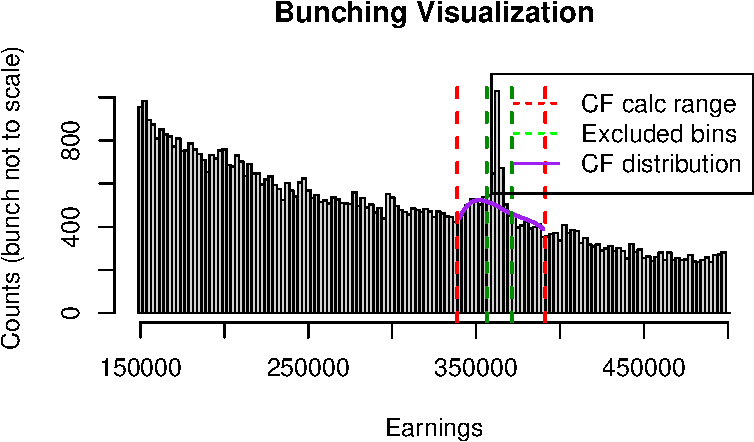
\includegraphics[keepaspectratio]{report_files/figure-pdf/unnamed-chunk-6-1.pdf}}

\begin{Shaded}
\begin{Highlighting}[]
\CommentTok{\# Estimate of the elasticity from the package}
\NormalTok{estim}\SpecialCharTok{$}\NormalTok{e}
\end{Highlighting}
\end{Shaded}

\begin{verbatim}
[1] 0.1318855
\end{verbatim}

\subsection{d.}\label{d.}

\begin{itemize}
\tightlist
\item
  Different: (1) setting the bunching width, (2) excluding bins, (3)
  polynomial order.
\end{itemize}

\section{Part 2}\label{part-2}

\subsection*{References}\label{references}
\addcontentsline{toc}{subsection}{References}

\phantomsection\label{refs}
\begin{CSLReferences}{1}{0}
\bibitem[\citeproctext]{ref-saez2010}
Saez, Emmanuel. 2010. {``Do Taxpayers Bunch at Kink Points?''}
\emph{American Economic Journal: Economic Policy} 2 (3): 180--212.
\url{https://doi.org/10.1257/pol.2.3.180}.

\end{CSLReferences}




\end{document}
